\documentclass[pdf,aspectratio=169]{beamer}
\usepackage[]{hyperref,graphicx,siunitx,lmodern,booktabs}
\usepackage{physics}
\usepackage{em-commands}
\mode<presentation>{\usetheme{EM}}

%Question Numbering
\newcounter{questionnumber}
\newcommand{\qnum}{%
	\stepcounter{questionnumber}%
	Q\arabic{questionnumber}
}
\resetcounteronoverlays{questionnumber}

\graphicspath{ {../Images/} }

\sisetup{per-mode=symbol}

%preamble
\title{Meeting at Laplace}
\date{September 24, 2018}
\author{Jed Rembold}

\begin{document}
\renewcommand{\theenumi}{\Alph{enumi}}

\begin{frame}{Announcements}
	\begin{itemize}
		\item Homework 4 due tonight!
		\item I'll try to have HW 5 out by tonight, tomorrow at latest
		\item For Wednesday read Ch 3.2, the Method of Images
		\item On Friday I'm aiming for a computer tutorial on the Method of Relaxation
	\end{itemize}
\end{frame}

\begin{frame}{\qnum}
	A neutral copper slab has several hollow patches in which live several charges, each with charge $+q$. What is the total charge on the outside surface of the copper slab?
	\begin{columns}
		\column{0.5\textwidth}
		\begin{center}
			\begin{tikzpicture}
				\draw[fill = orange!40, even odd rule] (0,0) rectangle +(5,4) (2,2) circle (1) (4,3) circle (0.5);
				\draw[fill=red!40] (2.5,2) circle (.25);
				\pic at (2.5,2) {plus};
				\draw[fill=red!40] (4,3) circle (.25);
				\pic at (4,3) {plus};
				\draw[<-] (5,1) -- +(30:.5) node[right,math] {q_{outer}};
			\end{tikzpicture}
		\end{center}
		\column{0.5\textwidth}
		\begin{enumerate}
			\item $q_{outer} = 0$
			\item \alert<2>{$q_{outer} = 2q$}
			\item $q_{outer} = -2q$
			\item $0 < q_{outer} < 2q$
		\end{enumerate}
	\end{columns}
\end{frame}

\begin{frame}{\qnum}
	A region of space contains no charges. What can you say about $V$ in the interior?
	\begin{columns}
		\column{0.5\textwidth}
		\begin{enumerate}
			\item $V(r)=0$ everywhere in the interior
			\item $V(r)=$ constant everywhere in the interior
			\item \alert<2>{Not much can be said. $V(r)$ has many possibilities in there}
		\end{enumerate}
		\column{0.5\textwidth}
		\begin{center}
			\begin{tikzpicture}[use Hobby shortcut]
				\draw[very thick, closed, tension=.800] (0,0) .. (3,1) .. (2,3) .. (0,1);
				\node[align=center] at (1.5,1) {$\rho=0$\\in here};
			\end{tikzpicture}
		\end{center}
		
	\end{columns}
\end{frame}

\begin{frame}{\qnum}
	What is the solution to Laplace's Equation in 1D if the boundaries are given by $V(x=\SI{0}{\m})=\SI{10}{\volt}$ and $V(x=\SI{10}{\m})=\SI{5}{\volt}$.
	\begin{enumerate}
		\item $V(x) = 2x$
		\item $\displaystyle V(x) = 2x + 10$
		\item \alert<2>{$\displaystyle V(x) = -\frac{x}{2}+10$}
		\item $\displaystyle V(x) = x^2 - \frac{21}{2}x + 10$
	\end{enumerate}
\end{frame}

\begin{frame}{\qnum}
	Which on the following height maps is a legitimate solution to the Laplace Equation?
	\onslide<2>{\alert{C is best!}}
	\begin{center}
		\includegraphics[width=\textwidth]{LaplacePlots.pdf}
		\includegraphics[width=\textwidth]{LaplaceColorbar.pdf}
	\end{center}
\end{frame}

\begin{frame}{\qnum}
	To solve the 1D Laplace Equation requires we submit 2 boundary conditions to solve for the two arbitrary constants. How many boundary conditions must we require for solving the 2D Laplace Equation?
	\begin{enumerate}
		\item Still 2. The Laplace equation always requires 2 boundary conditions.
		\item 4 different points on the boundary will suffice
		\item 2 points on the boundary and 2 derivatives at the boundary will suffice
		\item \alert<2>{None of the above will suffice}
	\end{enumerate}
\end{frame}

\begin{frame}{\qnum}
	A region of space contains no charges. The boundary also has $V=0$ everywhere along it. What can you say about $V$ in the interior?
	\begin{columns}
		\column{0.5\textwidth}
		\begin{enumerate}
			\item \alert<2>{$V(r)=0$ everywhere in the interior}
			\item $V(r)=$ constant $>0$ everywhere in the interior
			\item Still not much can be said. $V(r)$ has many possibilities in there
		\end{enumerate}
		\column{0.5\textwidth}
		\begin{center}
			\begin{tikzpicture}[use Hobby shortcut]
				\draw[very thick, closed, tension=.800] (0,0) .. (3,1) .. (2,3) .. coordinate[pos=0.5] (a) (0,1);
				\node[align=center] at (1.5,1) {$\rho=0$\\in here};
				\draw[<-, thick] (a) --+(135:.5) node[above] {$V=0$};
			\end{tikzpicture}
		\end{center}
		
	\end{columns}
\end{frame}

\begin{frame}{\qnum}
	\begin{columns}
		\column{0.5\textwidth}
		If you put a positive test charge in the exact center of the cube of charges to the right, would it be in stable equilibrium?
		\begin{enumerate}
			\item Yes
			\item \alert<2>{No}
			\item I don't remember what stable equilibrium means\ldots
		\end{enumerate}
		\column{0.5\textwidth}
		\begin{center}
			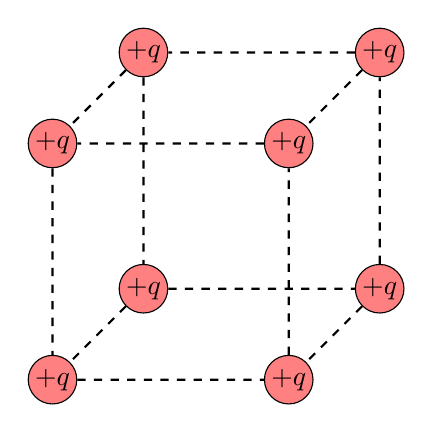
\begin{tikzpicture}[chg/.style={draw,circle,fill=red!50,inner sep=1pt}]
				\foreach \x in {0,3} {
					\foreach \y in {0,3}{
						\foreach \z in {0,3}{
							\node[chg] (\x\y\z) at (\x,\y,\z) {$+q$};
						}
					}
				}
				\draw[thick, dashed] (000) -- (300) -- (330) -- (030) -- (000)
									 (003) -- (303) -- (333) -- (033) --(003)
									 (000) -- (003)    (330) -- (333)
									 (300) -- (303)    (030) -- (033);
			\end{tikzpicture}
		\end{center}
		
	\end{columns}
\end{frame}


\end{document}
